\includeonlyframes{part1}

\lstset{
language=python,                             % Code langugage
basicstyle=\footnotesize,                   % Code font, Examples: \footnotesize, \ttfamily
keywordstyle=\color{OliveGreen},        % Keywords font ('*' = uppercase)
commentstyle=\color{gray},              % Comments font
%numbers=left,                           % Line nums position
numberstyle=\tiny,                      % Line-numbers fonts
stepnumber=1,                           % Step between two line-numbers
numbersep=0pt,                          % How far are line-numbers from code
backgroundcolor=\color{lightlightgray}, % Choose background color
frame=none,                             % A frame around the code
tabsize=1,                              % Default tab size
captionpos=b,                           % Caption-position = bottom
breaklines=true,                        % Automatic line breaking?
breakatwhitespace=false,                % Automatic breaks only at whitespace?
showspaces=false,                       % Dont make spaces visible
showtabs=false,                         % Dont make tabls visible
columns=flexible,                       % Column format
morekeywords={__global__, __device__,cudaMalloc,cudaMemcpy,vecAdd, <<<, >>>, cudaMemcpyHostToDevice, cudaMemcpyDeviceToHost, threadIdx, blockDim, blockIdx,texture,blocks,threads}  % CUDA specific keywords
}
\DeclareGraphicsExtensions{.pdf,.png,.gif}
\title[RSF School]{Developing your own \\programs in Madagascar}
\author[Jeffrey Shragge]{Jeffrey Shragge (with thanks to Jeff Godwin, CSM)}
\institute[CPGCO2, UWA]{Centre for Petroleum Geoscience and CO2 Sequestration \\University of Western Australia}
\vspace{-0.1\textheight}
\vspace{-0.1\textheight}
\date{July 22, 2011}

\def\radius{0.96cm}
\def\innerradius{0.85cm}

\frame[label=part1]{\titlepage}

%%%%%%%%%%%%%%%%%%%%%%%%%%%%%%%%%%%%%%%%%%%%%%%%%%%%%%%%%%%%%%%%%%
\setcounter{section}{1}

\part{Part I - Introduction}
 
\frame[label=part1]{
\frametitle{Writing / adding your own codes}
\begin{columns}
\begin{column}{0.45\textwidth}

\begin{block}{Isn't there a lot there already?!?}
\begin{itemize}
 \item There are $>$ 850 programs already in Madagascar
 \item Includes both seismic and non-seismic tools
 \item Incorporates generic data manipulation tools
  \end{itemize}
 \end{block}
\end{column}

\begin{column}{0.45\textwidth}

\uncover<2->{ 
\begin{block}{Yes! But not everything!}
\begin{itemize}
 \item Some tasks not easily doable with existing tools
 \item Some tools might not exist at all (i.e. your research!)
 \item Include some existing tools with your programs
  \end{itemize}
 \end{block}
}

\end{column}

\end{columns}
 }

%%%%%%%%%%%%%%%%%%%%%%%%%%%%%%%%%%%%%%%%%%%%%%%%%%%%%%%%%%%%%%%%%%
 
\frame[label=part1]{
\frametitle{Where to begin?}
\begin{columns}
\begin{column}{0.45\textwidth}

\begin{block}{Should you build programs for all of your needs?}
\centering
\begin{huge}
NO!
\vspace{-0.2cm}
\begin{figure}
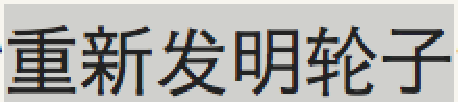
\includegraphics[width=0.7\textwidth]{./Fig/InventWheelChinese} 
\end{figure}
\vspace{-0.25cm}
\begin{figure}
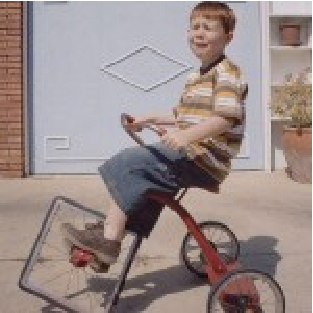
\includegraphics[width=0.7\textwidth]{./Fig/WHEEL} 
\end{figure}
\end{huge}
\end{block}
 \end{column}

\uncover<2->{

\begin{column}{0.45\textwidth}
Examples of ``Wheel'' programs
\begin{itemize}
\item Matrix multiply
\item Dataset concatenation
\item FFTs,  
\item Bandpass filtering
\item ...
\end{itemize}
}

\end{column}
\end{columns}
 }

%%%%%%%%%%%%%%%%%%%%%%%%%%%%%%%%%%%%%%%%%%%%%%%%%%%%%%%%%%%%%%%%%%
 
\frame[label=part1]{
\frametitle{Standing on the shoulders of giants ...}
\begin{columns}
\begin{column}{0.9\textwidth}


\begin{block}{Make sure to check out ...}
\centering
\vspace{0.25cm}
\begin{huge}
{\bf sfdoc -k .}
\end{huge}
\vspace{0.25cm}
\end{block}

\begin{block}{Where to begin ...}
\begin{itemize}
 \item Focus your time / energy on doing YOUR new research!
 \item Do not waste time reinventing things 
 \item Look at existing Madagascar programs for help
 \begin{itemize}
 \item \$RSFROOT/RSFSRC/book/Recipes
 \item \$RSFROOT/RSFSRC/user/
 \item  User / Developer mailing lists
 \end{itemize}
  \end{itemize}
 \end{block}
 
\end{column}
\end{columns}
 }

%%%%%%%%%%%%%%%%%%%%%%%%%%%%%%%%%%%%%%%%%%%%%%%%%%%%%%%%%%%%%%%%%%
 
\frame[label=part1]{
\frametitle{Presentation Goals}
\begin{columns}
\begin{column}{0.9\textwidth}


\begin{block}{What is the main goal of this tutorial?}
\centering
\vspace{0.25cm}
\begin{large}
After this presentation you should know how to put your own programs into Madagascar
\end{large}
\vspace{0.25cm}
\end{block}

\begin{block}{How are we going to do it?}
\begin{enumerate}
 \item Finish coding a ``Vector Addition'' program
 \item Compile and Install it in RSF
 \item Test it with various SConstruct Flow() and Plot() rules
 \end{enumerate}
 \end{block}
 
\end{column}
\end{columns}
 }


%%%%%%%%%%%%%%%%%%%

\frame [ label=part1] {
\frametitle{Agenda}
\begin{columns}
\begin{column}{0.9\textwidth}
\begin{large}
This talk will focus on:
\vspace{0.25cm}
\begin{enumerate}
\item When should I start adding my own codes?
\item Madagascar's API
\item RSF program structure
\item Assignment 1: Vector Addition
\end{enumerate}
\end{large}

\end{column}
\end{columns}
}

%%%%%%%%%%%%%%%%%%%

\frame [ label=part1] {
\frametitle{Agenda}
\begin{columns}
\begin{column}{0.9\textwidth}
\begin{large}
This talk will focus on:
\vspace{0.25cm}
\begin{enumerate}
\item When should I start adding my own codes?
\color{gray}
\item Madagascar's API
\item RSF program structure
\item Assignment 1: Vector Addition
\color{black}
\end{enumerate}
\end{large}

\end{column}
\end{columns}
}

%%%%%%%%%%%%%%%%%%%%%%%%%%%%%%%%%%%%%%%%%%%%%%%%%%%%%%%%%%%%%%%%%%
 
\frame[label=part1]{
\frametitle{Where to draw the line with development}
\begin{columns}
\begin{column}{0.9\textwidth}

\begin{block}{Program architecture goals}
RSF programs are task-centric:
\begin{itemize}
\item Each program performs one task or a common task set:
\begin{itemize}
\item Spray (Forward operator)
\item Stack (Adjoint operator)
\end{itemize}
\item Programs constructed to run in a \structure{pipeline} with input from standard in and output to standard out:
\begin{itemize}
\item $<$ in.rsf sf\_my\_program $>$ out.rsf 
\item $<$ in.rsf $\vert$ sfwindow $\vert$ sf\_my\_program $\vert$ sfwindow $>$ out.H
\end{itemize}
\item Pass parameters from:
\begin{itemize}
\item Command line or SConstruct file (in rule or in dictionary)
\end{itemize}
\end{itemize}
\end{block}

\end{column}
\end{columns}
 }

%%%%%%%%%%%%%%%%%%%%%%%%%%%%%%%%%%%%%%%%%%%%%%%%%%%%%%%%%%%%%%%%%%
 
\frame[label=part1]{
\frametitle{Where to draw the line with development}
\begin{columns}
\begin{column}{\textwidth}

Zhang wants to apply the newest XYZ filter in the frequency domain: ${\bf L}(\omega)$.  However, his RSF data is in the time domain ${\bf d}(t)$. How should Zhang design his new RSF program to obtain filtered data ${\bf d}_{filt}(t)$? \\
\vspace{0.2cm}
\uncover<2->{
Use a solution that involves FFT pair ${\bf F}(t\rightarrow\omega)$ and ${\bf F}^{-1}(\omega\rightarrow t)$:
\begin{equation}
{\bf d}_{filt} = {\bf F}^{-1}{\bf L}{\bf F} {\bf d}
\end{equation}
}
\vspace{0.2cm}
\uncover<3->{Let us explore 3 solutions:}
\begin{enumerate}
\uncover<4->{ 
\item Write new code that applies ${\bf F}$, then ${\bf L}$, and then ${\bf F}^{-1}$. 
}
\uncover<5->{ 
\item Write new code that applies ${\bf L}$, but calls an existing library for ${\bf F}$ and ${\bf F}^{-1}$. 
}
\uncover<6->{
\item Write an ${\bf L}$ filter program.  Use Madagascar to apply  ${\bf F}$ and ${\bf F}^{-1}$. 
}
\end{enumerate} 
 
\end{column}
\end{columns}
 }



%%%%%%%%%%%%%%%%%%%%%%%%%%%%%%%%%%%%%%%%%%%%%%%%%%%%%%%%%%%%%%%%%%
 
\frame[label=part1]{
\frametitle{Thinking about program design}
\begin{columns}
\begin{column}{0.475\textwidth}
  
\begin{block}{Three possible solutions}
\begin{enumerate}
\item Zhang writes code that applies ${\bf F}$, then ${\bf L}$, and then ${\bf F}^{-1}$.
\vspace{0.38cm}
\uncover<2->{\item Zhang writes a new code that applies ${\bf L}$, and calls existing libraries for ${\bf F}$ and ${\bf F}^{-1}$}
\vspace{0.38cm}
\uncover<3->{\item Zhang writes an ${\bf L}$ filter program, and uses Madagascar to apply  ${\bf F}$ and ${\bf F}^{-1}$ }
\end{enumerate} 
\end{block}
  \end{column}

\begin{column}{0.475\textwidth}
 \begin{block}{\color{blue}Pros \color{white} and \color{red} Cons \color{black}}
\begin{enumerate}
\item \color{red}Not task-centric and Zhang wastes time researching / writing / debugging a FFT code.   

\uncover<2->{\item \color{red} Not task-centric \color{blue} but Zhang uses existing libraries to shorten development time. \color{black}
}
\uncover<3->{\item \color{blue} Task-centric coding that can be used in a pipeline, and be applied to any frequency domain data set.\color{black}
}

\end{enumerate} 
\end{block}
\end{column}
\end{columns}
 }




%%%%%%%%%%%%%%%%%%%

\frame [ label=part1] {
\frametitle{Agenda}
\begin{columns}
\begin{column}{0.9\textwidth}

This talk will focus on:
\vspace{0.25cm}
\begin{large}
\begin{enumerate}
\item When should I start adding my own codes?
\item Madagascar's API
\color{gray}
\item RSF program structure
\item Assignment 1: Vector Addition (25 mins)
\color{black}
\end{enumerate}
\end{large}

\end{column}
\end{columns}
}



%%%%%%%%%%%%%%%%%%%%%%%%%%%%%%%%%%%%%%%%%%%%%%%%%%%%%%%%%%%%%%%%%%
 
\frame[label=part1]{
\frametitle{RSF framework}
\begin{columns}
\begin{column}{0.6\textwidth}

\only<1>{
Application Programming Interface (API) 
\begin{itemize}
\item A set of rules or interface that software programs follow to communicate with each other
\vspace{0.4cm}
\item Specifies routines, data structures and the protocols used for communicate between the consumer program and the implementer program of the API
\end{itemize}
}
\only<2>{
Madagascar has a number of APIs
\begin{itemize}
\item C/C++
\item Python
\item Fortran 77
\item Fortran 90
\item Matlab
\item Java
\item Octave
\end{itemize}
}
\end{column}

\begin{column}{0.4\textwidth}
\only<1->{
\begin{figure}
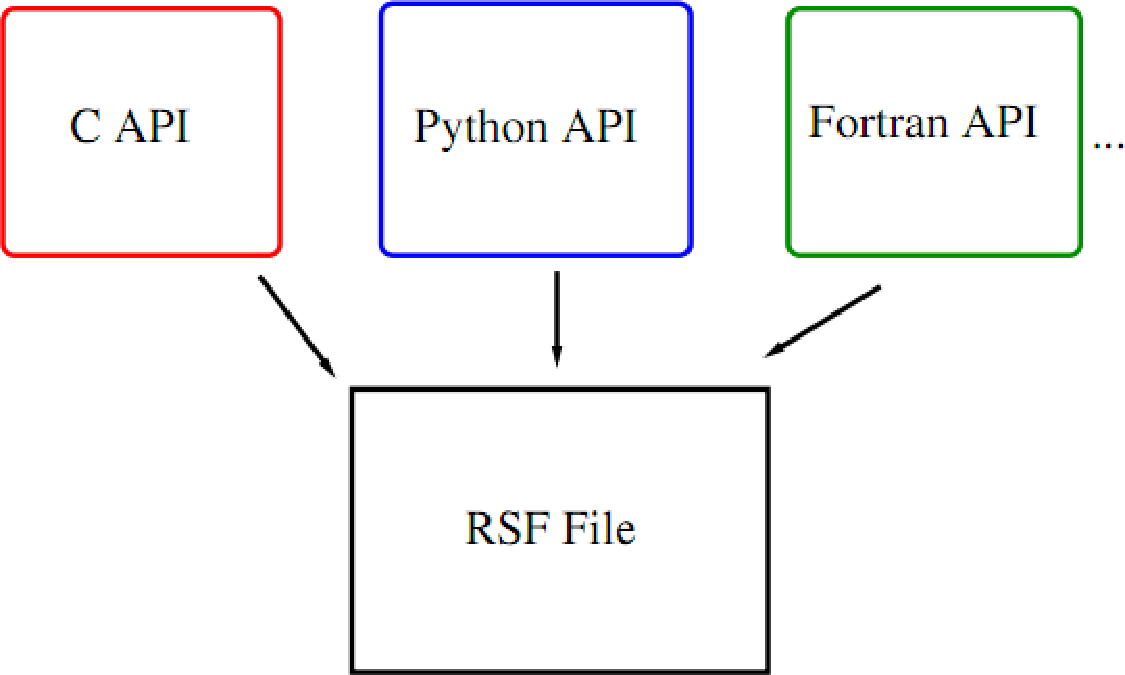
\includegraphics[width=\textwidth]{./Fig/RSF_FRAMEWORK} 
\vspace{0.2cm}
\end{figure}
  }
\end{column}


\end{columns}
 }


%%%%%%%%%%%%%%%%%%%%%%%%%%%%%%%%%%%%%%%%%%%%%%%%%%%%%%%%%%%%%%%%%%
 
\frame[label=part1]{
\frametitle{Overview of the C API }
\begin{columns}
\begin{column}{0.6\textwidth}
Strength of Madagascar API (here C):
\begin{itemize}
\uncover<1->{
\item  \structure{Interoperable}: 
\begin{itemize}
\item Common RSF file structure
\item Defines standard for data exchange
\item Enables pipelining with other programs
\end{itemize}
}
\uncover<2->{
\item Improves \structure{development efficiency}
\begin{itemize}
\item Access RSF C functions / libraries
\item \structure{Encapsulate} many tasks (e.g. predefined data I/O subroutines)
\end{itemize}
}
\uncover<3->{
\item Enhances \structure{usability}
\begin{itemize}
\item Common program documentation style
\item Helps other people use your code
\item Helps you use other people's code
\end{itemize}
}
\end{itemize}

\end{column}


\begin{column}{0.4\textwidth}
\begin{figure}
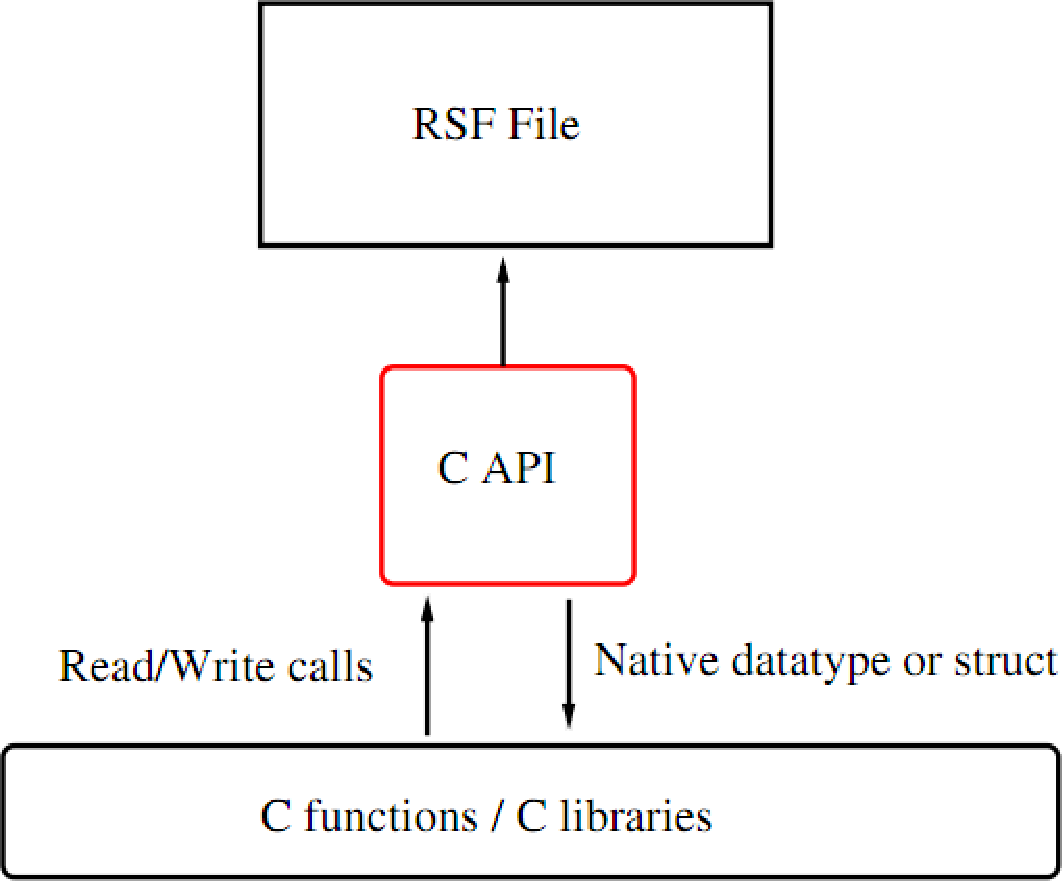
\includegraphics[width=\textwidth]{./Fig/API_OVERVIEW} 
\vspace{0.2cm}
\end{figure}
\end{column}

\end{columns}
 }
 
%%%%%%%%%%%%%%%%%%%

\frame [ label=part1] {
\frametitle{Agenda}
\begin{columns}
\begin{column}{0.9\textwidth}

This talk will focus on:
\vspace{0.25cm}
\begin{large}
\begin{enumerate}
\item When should I start adding my own codes?
\item Madagascar's API
\item RSF program structure
\color{gray}
\item Assignment 1: Vector Addition (25 mins)
\color{black}
\end{enumerate}
\end{large}

\end{column}
\end{columns}
}

%%%%%%%%%%%%%%%%%%%%%

\begin{frame}[ label=part1,fragile]
\frametitle{RSF Clipit Example (F90) }

Geophysical task: Clip 1D data set where greater than user defined value.

%\href{http://www.ahay.org/wiki/Guide_to_madagascar_API}

\begin{columns}
\begin{column}{0.5\textwidth}
\begin{lstlisting}
!! STEP 1 - Documentation
program Clipit	
!! STEP 2 - Import RSF API
  use rsf  
  
  implicit none
  type (file)  :: in, out
  integer  :: n1, n2, i1, i2
  real  :: clip
  real, dimension(:), allocatable :: trace
 
 !! STEP 3 - Initialize RSF command line parser
  call sf_init()        
  
  !! STEP 4 - Read command line variables
  call from_par("clip",clip)
   - 
  !! STEP 5 - Declare all input / output RSF files
  in = rsf_input(); out = rsf_output()

\end{lstlisting}

\end{column}

\begin{column}{0.5\textwidth}
\begin{lstlisting}  
!! STEP 6 - Read input data headers
  call from_par(in,"n1",n1)
  
!! STEP 7 - Write output data headers
  call to_par(out,"n1",n1)
  
  n2 = filesize(in,1)
  allocate (trace (n1))
 
  do i2=1, n2                ! loop over traces
     !! STEP 8 - Read input data sets
     call rsf_read(in,trace) !! STEP 7

     !! STEP 9 - Do ``geophysics''
     where (trace >  clip) trace =  clip
     where (trace < -clip) trace = -clip

     !! STEP 10 - Write output  data sets
     call rsf_write(out,trace)
  end do
end program Clipit
\end{lstlisting}

\end{column}

\end{columns}
\end{frame}
 
%%%%%%%%%%%%%%%%%%%%%

\begin{frame}[ label=part1,fragile]
\frametitle{Generic RSF program}
\begin{columns}
\begin{column}{0.55\textwidth}
\begin{enumerate}
\item<1-| alert@1> Documentation (comments)
\item<1-| alert@2> Import RSF API
\item<1-| alert@3> Initialize RSF command line parser
\item <1-| alert@4>Read command line variables
\item <1-| alert@5>Declare all input / output RSF files
\item <1-| alert@6>Read input data headers
\item <1-| alert@7>Create output data headers
\item <1-| alert@8>Read input data sets
\item <1-| alert@9>(Do geophysics)...
\item <1-| alert@10>Write output data  
\end{enumerate}
\end{column}

\begin{column}{0.45\textwidth}
\color{red}
\only<1> {!! STEP 1\\! Clipit - Program to clip a traces\\}
\only<2> {!! STEP 2\\use rsf\\}
\only<3> {!! STEP 3\\call sf\_init()\\}
\only<4> {!! STEP 4\\call from\_par("clip",clip)\\}
\only<5> {!! STEP 5\\ in = rsf\_input();\\ out = rsf\_output()\\}
\only<6> {!! STEP 6\\ call from\_par(in,"n1",n1)\\}
\only<7> {!! STEP 7\\ call to\_par(out,"n1",n1)\\}
\only<8> {!! STEP 8\\ call rsf\_read(in,trace)}
\only<9> {!! STEP 9\\where (trace $>$  clip) trace =  clip\\}
\only<10> {!! STEP 10\\ call rsf\_write(out,trace)\\}
\color{black}

\end{column}
\end{columns}
\end{frame}
 


%%%%%%%%%%%%%%%%%%%

\frame [ label=part1] {
\frametitle{Agenda}
\begin{columns}
\begin{column}{\textwidth}

This talk will focus on:
\vspace{0.25cm}
\begin{large}
\begin{enumerate}
\item When should I start adding my own codes?
\item Madagascar's API
\item RSF program structure
\item Assignment 1: Vector Addition
\end{enumerate}
\end{large}

\end{column}
\end{columns}
}
%%%%%%%%%%%%%%%%%%%%%

\frame   [ label=part1]   {
\frametitle{Part 1: Building your program}
\begin{columns}
\begin{column}{\textwidth}
\begin{enumerate}[1]
\item Take your copy of SCHOOL\_CODE.tgz and do:  
\begin{itemize}
\begin{footnotesize}
\item cp SCHOOL\_CODE.tgz \$RSFROOT/RSFSRC/user/; cd  \$RSFROOT/RSFSRC/user/;
\item tar -xcvf SCHOOL\_CODE.tgz;
\end{footnotesize}
\end{itemize}
\vspace{0.2cm}
\item You have a copy of an {\bf almost finished} ``vector addition'' code in C
\begin{itemize}
\item \$RSFROOT/RSFSRC/user/school/Mvectoradd\_C.c
\end{itemize}
Your assignment is to put the ``geophysics'' into the vector addition code.  Open the file in a text editor and complete the C=A+B assignment.  
\begin{itemize}
\item Hint: Vector index in F90 is A(); Vector index in C is A[].
\end{itemize}
\vspace{0.2cm}
\item After completing this task build the code in the local directory by:
\begin{itemize}
\item Type: {\bf scons sfvectoradd\_C}
\end{itemize}
\vspace{0.2cm}
\item Install the C files (not yet F90?) into \$RSFROOT/bin/ by 
\begin{itemize}
\item Type: {\bf cd \$RSFROOT/RSFSRC/ ; scons install}
\end{itemize}
\end{enumerate}
\end{column}

\end{columns}
} 

%%%%%%%%%%%%%%%%%%%%%

\frame   [ label=part1]   {
\frametitle{Part 2: Testing your program}
\begin{columns}
\begin{column}{\textwidth}
\begin{enumerate}
\item[5] Take your copy of SCHOOL\_TEST.tgz and do:  
\begin{itemize}
\begin{footnotesize}
\item cp SCHOOL\_TEST.tgz /path/to/work/dir/; cd /path/to/work/dir/;
\item tar -xcvf SCHOOL\_TEST.tgz
\end{footnotesize}
\end{itemize}
You have an incomplete {\bf SConstruct} file in ./school\_test/.   We have to add lines into this file in order to test our {\bf sfvectoradd\_C} programs.
\vspace{0.2cm}
\item[7] Create two random vectors {\bf A} and {\bf B} (of the same length) to add.  Create these with a Madagascar program in the provided {\bf Flow()} rule.
\begin{itemize}
\item Hint: there is more than 1 answer: {\bf sfdoc -k .}
\item Build the Flow() rule for A and B by: {\bf scons A.rsf; scons B.rsf}
\end{itemize}
\vspace{0.2cm}
\item [8] You must obtain {\bf C} from {\bf A} and {\bf B}.  Do this by: {\bf scons C\_C.rsf}		
\vspace{0.2cm}
\item[9] Do you know that you got the correct answer? Let's test our program against a (correct) Madagascar one: {\bf sfmath}.  Look at the {\bf sfmath} self-doc page to find out how to complete the provided {\bf Flow()} rule.
\begin{itemize}
\item Hint: there is more than 1 answer: {\bf sfdoc -k .}
\item Build example by: {\bf scons Ctest\_C.rsf}
\end{itemize}
\vspace{0.2cm}
\end{enumerate}
\end{column}

\end{columns}
} 
